\lecture{12}{Thu 08 Feb '24}{}
\chapter{Context-Free Grammars} \label{ch:cfg}
\section{Introduction}
The syntax of regular expressions over an alphabet $\set{a, b}$ is defined
by \[
    r ::= \O \mid a \mid b \mid r + r \mid r \cdot r \mid r^*.
\] This is an example of a context-free grammar (CFG).
Context-free grammars arise enaturally in syntax of programming language,
parsing, compiling.

\begin{examples}
    \item $G_1$ is the grammar given by the rules \begin{align*}
        S &\to aX \\
        X &\to aX \\
        X &\to bX \\
        X &\to b
    \end{align*}
    A string is derived from these rules as follows:
    Begin with $S$ and keep rewriting the current string by replacing a
    non-terminal with the right-hand side in a production rule.
    For example, \[
        S \to aX \to abX \to abb.
    \] The language defined by a grammer $G$, written $L(G)$,
    is the set of all terminal strings that can be generated by $G$. \\
    The language generated by $G_1$ is $a(a+b)^*b$.
    \item $G_2$ is the grammar given by the rules \begin{align*}
        S &\to aSb \\
        S &\to \epsilon
    \end{align*}
    An example string in this grammer is \[
        S \to aSb \to aaSbb \to aaaSbbb \to aaabbb
    \] and $L(G) = \set{a^nb^n \mid n \ge 0}$.
    Suppose we add the rule $S \to bSa$.
    We write this in short as \[
        S \to aSb \mid bSa \mid \epsilon.
    \] The language generated by this grammar is all even length
    ``inverse'' palindromes, \ie, the mirror image of any alphabet about the
    midpoint inverts $a$'s to $b$'s and vice versa.
    \item Let $G_3$ be given be \[
        S \to aSa \mid bSb \mid a \mid b \mid \epsilon.
    \] Then $L(G_3)$ is all palindromes.
    \item Let $G_4$ be given by \[
        S \to (S) \mid SS \mid \epsilon.
    \] This gives the language of all balanced parentheses.
    Formally, a $w \in \{\texttt{(}, \texttt{)}\}$ is balanced if
    \begin{itemize}
        \item $\#_((w) = \#_)(w)$, and
        \item for each prefic $u$ of $w$, $\#_((u) \ge \#_)(u)$.
    \end{itemize}
    \begin{exercise}
        Derive the string $((()())()())$ from $G_4$.
    \end{exercise}
    \begin{solution}
        \begin{align*}
            S &\to (S) \\
            &\to (SS) \\
            &\to ((S)S) \\
            &\to ((SS)SS) \\
            &\to (((S)(S))(S)(S)) \\
            &\to ((()())()())
        \end{align*}
    \end{solution}
    One can visualise any balanced string $w$ as a graph of points
    $(n, \delta)$, where $0 \le n \le \abs{w}$ and $\delta$ is the
    difference between the number of left and right parentheses in the
    prefix of $w$ of length $n$.
    The graph starts at $(0, 0)$ and ends at $(\abs{w}, 0)$,
    and never goes below the $x$-axis.
    \begin{center}
        %pgfplots
        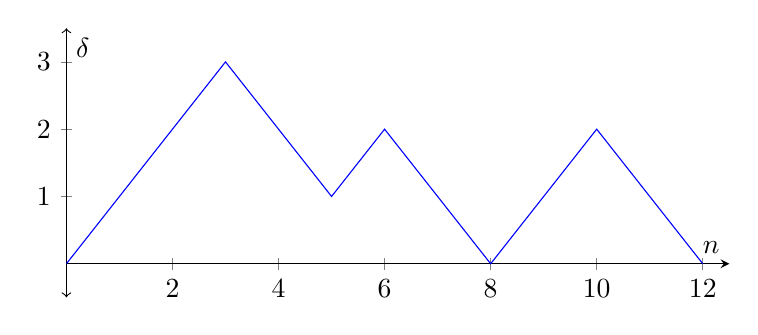
\begin{tikzpicture}
            \begin{axis}[
                axis lines = center,
                y axis line style = {<->},
                xlabel = $n$,
                ylabel = $\delta$,
                xmin = 0,
                xmax = 12.5,
                ymin = -0.5,
                ymax = 3.5,
                height = 5cm,
                width = 10cm,
            ]
            \addplot+ [no markers] coordinates {
                    (0, 0)
                    (3, 3)
                    (5, 1)
                    (6, 2)
                    (8, 0)
                    (10, 2)
                    (12, 0)
                };
            \end{axis}
        \end{tikzpicture}
    \end{center}
\end{examples}

\begin{definition}[Context-free grammar] \label{def:cfg}
    A Context-Free Grammar (CFG) is a 4-tuple $G = (N, A, S, P)$, where
    \begin{itemize}
        \item $N$ is a finite set of \emph{non-terminal symbols},
        \item $A$ is a finite set of \emph{terminal symbols}
        disjoint from $N$,
        \item $S \in N$ is the non-terminal \emph{start symbol}, and
        \item $P$ is a finite subset of $N \times (N \cup A)^*$,
        called the set of \emph{productions} or \emph{rules}.
        A production $(X, \alpha)$ is written as $X \to \alpha$.
    \end{itemize}
\end{definition}
We will denote letters with lower-case letters, non-terminals with
upper-case letters, and strings of both letters and non-terminals with
Greek letters.
\begin{definition}
    Given a CFG $G = (N, A, S, P)$, we define the relation $\xRightarrow{n}$
    on $(N \cup A)^*$ inductively as follows:
    \begin{itemize}
        \item $\alpha \xRightarrow{0} \alpha$;
        \item $\alpha \xRightarrow{1} \beta$ if $\alpha$ is of the form
        $\alpha_1 X \alpha_2$ and $X \to \gamma$ is a production rule such
        that $\beta = \alpha_1 \gamma \alpha_2$; and
        \item $\alpha \xRightarrow{n+1} \beta$ if there exists a string
        $\gamma$ such that $\alpha \xRightarrow{n} \gamma$ and
        $\gamma \xRightarrow{1} \beta$.
    \end{itemize}
    We further define $\Rightarrow^*_G$ as the union of all
    $\xRightarrow{n}$ for $n \in \N$.

    A \emph{sentential form} of $G$ is any $\alpha \in (N \cup A)^*$ such
    that $S \Rightarrow^*_G \alpha$.

    The language defined by $G$ is
    $L(G) = \set{w \in A^* \mid S \Rightarrow^*_G w}$.
\end{definition}

\section{Parse Trees} \label{sec:cfg:parse_trees}
Each derivation of a string $w$ from a CFG $G$ can be represented by a
parse tree, where each internal node is labelled by a non-terminal and
each leaf is labelled by a terminal or $\epsilon$.
Each internal node has children corresponding to the right-hand side of
a production rule for the non-terminal label of the node.

The string represented by a parse tree is the concatenation of the
labels of the leaves read from left to right.

\begin{exercise}
    Consider $G_1$ given in the examples above. \begin{align*}
        S &\to aX \\
        X &\to aX \mid bX \mid b
    \end{align*}
    Prove that $L(G_1) = a(a + b)^*b$.
\end{exercise}
\begin{proof}
    Let $P(n)$ be that for any $w \in (N \cup A)^*$, $S \xRightarrow{n} w$
    if and only if \[
        w \in a(a + b)^{n-1}X + a(a + b)^{n-2}b,
    \] where we consider the second term to be $\O$ if $n < 2$.
    The case $n = 1$ is direct.

    Suppose $P(k)$ holds.
    Let $w \in (N \cup A)^*$.
    Then $S \xRightarrow{k+1} w$ iff there is some $\alpha$ such that
    $S \xRightarrow{k} \alpha$ and $\alpha \xRightarrow{1} w$.
    By the induction hypothesis, this is iff $\alpha \in a(a+b)^{k-1}X
    + a(a+b)^{k-2}b$ and $\alpha \xRightarrow{1} w$.
    Since the second term has no non-terminals, this is equivalent to
    $\alpha \in a(a+b)^{k-1}X$ and $\alpha \xRightarrow{1} w$ so
    \begin{align*}
        w &\in a(a+b)^{k-1}aX + a(a+b)^{k-1}bX + a(a+b)^{k-1}b \\
        &= a(a+b)^k X + a(a+b)^{k-1}b
    \end{align*}
    Thus $P(k+1)$ holds.

    By induction, $P(n)$ holds for all $n \in \N$.
    Then $L(G_1) = \set{w \in A^* \mid S \Rightarrow^*_G w}$ is the union
    of $a(a+b)^{n-2}b$ which is $a(a+b)^*b$.
\end{proof}
